% asjcdoc.tex V1.0, 7 July 2008

\documentclass[times]{asjcauth}

\usepackage{moreverb}
\usepackage{graphicx}
\usepackage{verbatim}
\usepackage{amsmath}
\usepackage{amsfonts}
\usepackage{array}
\usepackage{enumerate}
\usepackage{endfloat}
\usepackage{url}
\usepackage{psfrag}
\usepackage{times}
\usepackage{amssymb}
\usepackage{amstext}
\usepackage{mathrsfs}
\usepackage{epsfig}
\usepackage{epstopdf}

%\usepackage[dvips,colorlinks,bookmarksopen,bookmarksnumbered,citecolor=red,urlcolor=red]{hyperref}

\newcommand{\mysmall}{\fontsize{7.5pt}{8pt}\selectfont}

\def\volumeyear{2008}
%\def\volumenumber{00}
%\def\DOI{asjc.000}

\begin{document}

\runninghead{A.~N.~Other: A Demonstration of the \emph{Asian J.
Contr.} Class File}

\categorytitle{Demonstration}

\title{A DEMONSTRATION OF THE \LaTeXe\ CLASS FILE FOR THE\\
\itshape{ASIAN JOURNAL OF CONTROL}\/\footnotemark[2]}

\author{A.~N.~Other}

\address{The author is with the Journals Production Department, John Wiley \& Sons, Ltd,
The Atrium, Southern Gate, Chichester, West Sussex, PO19~8SQ, UK.}

\received{July 8, 2008.}

\acks{This class file was developed by Sunrise Setting Ltd,
Torquay, Devon, UK. Website:
\href{http://www.sunrise-setting.co.uk}{\texttt{www.sunrise-setting.co.uk}}}

\begin{abstract}
This paper describes the use of the \LaTeXe\ \textsf{asjcauth.cls}
class file for setting papers for the \emph{Asian Journal of
Control}.
\end{abstract}

\keywords{\emph{Asian J. Contr.}, class file, \LaTeXe.}

\maketitle

\footnotetext[2]{Please ensure that you use the most up to date
class file,
available from the ASJC Home Page at\\
\href{http://www3.interscience.wiley.com/journal/117933310/home}{\mysmall\texttt{www3.interscience.wiley.com/journal/117933310/home}}}

\section{INTRODUCTION}
Many authors submitting to research journals
use \LaTeXe\ to prepare their papers. This paper describes the
\textsf{asjcauth.cls} class file which can be used to convert
articles produced with other \LaTeXe\ class files into the correct
form for publication in the \emph{Asian Journal of Control}.

The \textsf{asjcauth.cls} class file preserves much of the
standard \LaTeXe\ interface so that any document which was
produced using the standard \LaTeXe\ \textsf{article} style can
easily be converted to work with the \textsf{asjcauth} style.
However, the width of text and typesize will vary from that of
\textsf{article.cls}; therefore, \emph{line breaks will change}
and it is likely that displayed mathematics and tabular material
will need re-setting.

In the following sections we describe how to lay out your code to
use \textsf{asjcauth.cls} to reproduce the typographical look of
the \emph{Asian Journal of Control}. However, this paper is not a
guide to using \LaTeXe\ and we would refer you to any of the many
books available (see, for example, \cite{R1,R2,R3}).

\section{THE THREE GOLDEN RULES} Before we proceed, we would like to
stress \emph{three golden rules} that need to be followed to
enable the most efficient use of your code at the typesetting
stage:
\begin{enumerate}
\item[(i)] keep your own macros to an absolute minimum;

\item[(ii)] as \TeX\ is designed to make sensible spacing
decisions by itself, do \emph{not} use explicit horizontal or
vertical spacing commands, except in a few accepted (mostly
mathematical) situations, such as \verb"\," before a
differential~d, or \verb"\quad" to separate an equation from its
qualifier;

\item[(iii)] follow the \emph{Asian Journal of Control}
reference style.
\end{enumerate}

\begin{figure*}
\setlength{\fboxsep}{0pt}%
\setlength{\fboxrule}{0pt}%
\begin{center}
\begin{boxedverbatim}
\documentclass[times]{asjcauth}
%\documentclass[times,doublespace]{asjcauth}%For paper submission

\begin{document}

\runninghead{<Initials and Surnames>: <Short title>}

%\categorytitle{Brief Paper}

\title{<ALL CAPITALS>}

\author{<An Author, Someone Else, and Perhaps Another>}

\address{<The author(s) is (are) with <author's address(es)>}

\received{<Article history>}

%\acks{<Acknowledgements as appropriate>}

\begin{abstract}
<Text>
\end{abstract}

\keywords{<Key words separated by commas>}

\maketitle

\section{INTRODUCTION}
.
.
.
\end{boxedverbatim}
\end{center}
\caption{Example header text.\label{F1}}
\vspace{12pt}
\end{figure*}

\section{GETTING STARTED} The \textsf{asjcauth} class file should run
on any standard \LaTeXe\ installation. If any of the fonts, class
files or packages it requires are missing from your installation,
they can be found on the \emph{\TeX\ Live} CD-ROMs or from CTAN.

\emph{Asian Journal of Control} is published using Times fonts and
this is achieved by using the \verb"times"
option as\\
\verb"\documentclass[times]{asjcauth}".

\noindent If for any reason
you have a problem using Times you can easily resort to Computer
Modern fonts by removing the \verb"times" option.

\section{THE ARTICLE HEADER INFORMATION}
The heading for any file using \textsf{asjcauth.cls} is shown in
Fig.~\ref{F1}.

\subsection{Remarks}
\begin{enumerate}
\item[(i)] In \verb"\runninghead", keep the short title to no more
than 50 characters; use `\emph{et~al.}' if there are three or more
authors.

\item[(ii)] Please uncomment\\
\verb+\categorytitle{Brief Paper}+

\noindent if this is the category of paper you are submitting. Do not use
\verb+\categorytitle{...}+ for a regular paper.

\item[(iii)] Note that affiliations/addresses appear as a footnote.
Include correspondence e-mail address in brackets at the end.

\item[(iv)] For submitting a double-spaced manuscript, add
\verb"doublespace" as an option to the document\-class line.

\item[(v)] The abstract should be capable of standing by itself,
in the absence of the body of the article and of the bibliography.
Therefore, it must not contain any reference citations. \item[(v)]
Keywords are separated by commas.

\item[(vi)] Acknowledgements are included as a title page footnote.
\end{enumerate}

\section{THE BODY OF THE ARTICLE}

\subsection{Mathematics} \textsf{asjcauth.cls} makes the full
functionality of \AmS\/\TeX\ available. We encourage the use of
the \verb"align", \verb"gather" and \verb"multline" environments
for displayed mathematics.

\subsection{Two wheel robot model}

Call ${q}_{ci}$, ${\theta}_{i}$ are current position and orientation of the robot. ${v}_{ci}$ and ${\omega}_{i}$ are linear and angular velocity.
\begin{equation}
	\begin{split}
		&\dot{q}_{ci}=\left[
			\begin{array}{c}
			v_{ci}\cos(\theta_{i})\\
			v_{ci}\sin(\theta_{i})\\
			\end{array}
		\right],\\
		&\dot{\theta}_{i}=\omega_{i}
	\end{split}
\end{equation}
With
\begin{equation}
\mathbf{\dot{q}_{ci}}=\left[
		\begin{array}{c}
			v_{cx}\\
			v_{cy}\\
		\end{array}
	\right]
\end{equation}
Combining (1) and (2), we have: 
\begin{equation}
	\left[
		\begin{array}{c}
			v_{cx}\\
			v_{cy}\\
		\end{array}	
	\right]=
	\left[
		\begin{array}{cc}
			\cos(\theta_{i})&{0}\\
			\sin(\theta_{i})&{0}\\
		\end{array}		
	\right]
	\left[
		\begin{array}{c}
			v_{ci}\\
			\omega_{ci}\\
		\end{array}		
	\right],
\end{equation}
Where $v_{cx}$ and $v_{cy}$ are velocity of the center point of the robot in \textit{x-axis} and \textit{y-axis} of the \textit{global coordinate}. 
Calling:
\begin{equation}
{M}(\theta)=\left[\begin{array}{cc}
			\cos(\theta_{i})&{0}\\
			\sin(\theta_{i})&{0}\\
		\end{array}
		\right]
\end{equation}

In the discrete domain, we have: 
\begin{equation}
	\frac{q_{i}(t+1)-q_{i}(t)}{\Delta{t}}=
	{M}(\theta)\left[
		\begin{array}{c}
			v_{ci}\\
			\omega_{ci}\\
		\end{array}
	\right]
\end{equation}
Thus, 
\begin{equation}
	q_{i}(t+1)=q_{i}(t)+\Delta{t}M(\theta)\left[
		\begin{array}{c}
			v_{ci}\\
			\omega_{ci}\\
		\end{array}
		\right],
\end{equation}
\begin{equation}
\theta_{i}(t+1)=\theta_{i}(t)+\Delta{t}\omega_{i}(t)
\end{equation}
On other hand, call $v_{l}$ and $v_r$ are velocity of the left and right wheels of the robot, correspondingly, we have: 

\begin{equation}
	\begin{split}
		v_{ci}=\frac{v_l+v_r}{2} \\
		\omega_{ci}=\frac{v_l-v_r}{d_{w}}\\ 
	\end{split}
\end{equation}
With $d_{w}$ is the distance between two wheel.So: 
\begin{equation}
\left[
	\begin{array}{c}
		v_{ci}\\
		\omega_{ci}\\
	\end{array}
\right]=
\left[
	\begin{array}{cc}
		\frac{1}{2}&\frac{1}{2}\\
		\frac{1}{d_{w}}&\frac{-1}{d_{w}}\\
	\end{array}
\right]
\left[
	\begin{array}{c}
		v_l\\
		v_r\\
	\end{array}
\right]
\end{equation}
Shown in Figure 2 is the diagram for the two wheel mobile robot.

\begin{figure}
\centering
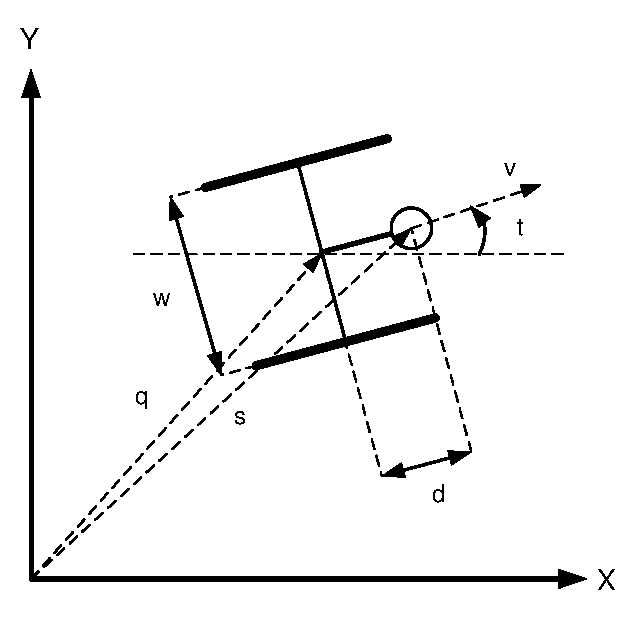
\includegraphics[width=.7\columnwidth]{Robot_kinematics.eps}
\caption{Robot's Kinematics}
\end{figure}

\subsection{Experiment setup}
\subsubsection{Mobile robot}

The mobile robot is depicted in Figure 3. The Arduino Mega board is used as the micro-controller, two wr703n router are used, one for streaming the video recorded from the web-cam equipped with paranormal lens, the other for receiving command remotely via the Internet. The overall control scheme is elaborated in Figure 4. There are three data collecting processes:
\begin{itemize}
\item The command sent to the Arduino board from the user is harvested at sampling time set to 50 milliseconds. However, due to the poor performance of the Arduino board, the actual sampling time fluctuates from 59 to 62 milliseconds. Thus,collapsing time between two samplings are recorded to be used in the simulation part.
\item The scene recorded by the paranormal web-cam is streamed on-line via the router, which can be accessible by the IP address of the router. The control program running in the control PC records the stream with 5 frame per second, e.g. 5 Hz.
\item The location of the mobile robot is tracked by the ceiling camera, by which it is updated with the same sampling rate as the streaming video.   
\end{itemize}

\begin{figure}
\centering
\includegraphics[width=.7\columnwidth]{mobileRobot.jpg}
\caption{Mobile Robot}
\end{figure}

\begin{figure}
\centering
\includegraphics[width=.7\columnwidth]{ControlFlow.pdf}
\caption{Overall Control Scheme}
\end{figure}

\subsubsection{Experiment environment}
The testing environment is depicted in Figure 5. Robot is controlled in opened-loop manner by user, while the paranormal recording the surrounding scene.Two PCs are used in the experiment, one for sending command signals to the robot, the other for processing the images from the ceiling camera for tracking robot's trajectory, and recording the scene streamed from the paranormal camera installed on the robot. 

\begin{figure}
\centering
\includegraphics[width=.7\columnwidth]{testingEnvironment.jpg}
\caption{Testing Environment}
\end{figure}

\subsection{mat-lab code explanation}
The command saved from the Arduino board is stored in \emph{huan} file. The real robot's trajectory \emph{in image frame coordinate} is exported in \emph{output.txt} file. The scene recorded from the paranormal camera is saved in \emph{record12115h08.avi} file.

The file \emph{robotTrackSimulation.m} simulates the robot model which is described in 5.1. The simulated result is converted to the coordinate in picture's frame by the camera matrix stored in the file \emph{calibmatrix.mat}. The trajectory then is processed through a second calibration by translation and scaling matrices to minimize the difference between the simulated and the real trajectory. The model is confirmed when the distance is sufficiently small.

The frames are queried from the video in the file \emph{frameQuery.m}. The experiment is executed in 112 seconds, e.g. sum of the sampling time from the command file and the length of the video is exactly matched. The command is sampled with 60 milliseconds sampling time, so there are 1852 sample points, which in turn are sub-sampled by factor of 1:4. Thus, there are \textbf{463} sub-sampling points. The video is recorded with 5 fps, so there are \textbf{558} frames for the video in total. The frames are numbered from 1 to 558. The sub-sampled command input is stored in the \textbf{commandSS} variable which is 463x3 matrix. The first two columns are the command input of linear velocity and angular velocity for the robot, correspondingly, the final column is exact time when a command was sent, in the time-line from 0 to 112.5 second. The variable \textbf{outPut} contains the real coordinate of the robot, sampled with frequency of 5Hz.  

The frames and the sub-sampled command are matched in following manner:

The time (in second) for each sample point in 463 sample points of the command is calculated in the time-line from 0 to 111 second, then it is projected to the frames set by following equation:

\begin{equation}
frame number=time\times\frac{558}{111}
\end{equation}  

The 463 sample frames are save in the \emph{frames} folder.

\subsection{Figures and tables} \textsf{asjcauth.cls} uses the
\textsf{graphicx} package for handling figures.

\newpage

Figures are called in as follows:
\begin{verbatim}
\begin{figure}
\centering
\includegraphics{<figure name>}
\caption{<Figure caption>}
\end{figure}
\end{verbatim}
Recall that the\\
\verb"\begin{figure*}...\end{figure*}"\\
commands are needed for a
figure spanning both columns.

For further details on how to size figures, etc., with the
\textsf{graphicx} package see, for example, \cite{R1}
or \cite{R3}. If figures are available in an
acceptable format (for example, .eps, .ps) they will be used but a
printed version should always be provided. \medbreak

%The standard coding for a table is shown in Fig.~\ref{F2}.
The standard coding for a table is as follows:

%\begin{figure}
%\setlength{\fboxsep}{0pt}%
%\setlength{\fboxrule}{0pt}%
%\begin{center}
%\begin{boxedverbatim}
\begin{verbatim}
\begin{table}
\caption{<Table caption>}
\centering
\begin{small}
\begin{tabular}{<table alignment>}
\toprule
<column headings>\\
\midrule
<table entries
(separated by & as usual)>\\
<table entries>\\
.
.
.\\
\bottomrule
\end{tabular}
\end{small}
\end{table}
\end{verbatim}
%\end{boxedverbatim}
%\end{center}
%\caption{Example table layout.\label{F2}}
%\end{figure}

\subsection{Cross-referencing}
The use of the \LaTeX\ cross-reference system
for figures, tables, equations, etc., is encouraged
(using \verb"\ref{<name>}" and \verb"\label{<name>}").

\subsection{Bibliography}
The normal commands for producing the reference list are:
\begin{verbatim}
\begin{thebibliography}{99}
\bibitem{<x-ref label>}
         <Reference details>
.
.
.
\end{thebibliography}
\end{verbatim}
where \verb"\bibitem{x-ref label}"
corresponds to \verb"\cite{x-ref label}" in the body of the article.
and \verb"{99}" is the widest such number expected and determines
the width of the number column in the reference list.

\subsection{Authors' biographies}
Please supply brief biographies for each of the authors. These
must be placed after the References. Please supply a recent
photograph of each author.

\subsection{Double spacing}
If you need to double space your document for submission please
use the \verb+doublespace+ option as shown in the sample layout in
Fig.~\ref{F1}.

\section{SUPPORT FOR \textsf{asjcauth.cls}}
We offer on-line support to participating authors. Please contact
us via e-mail at\\
\href{mailto:asjcauth-cls@wiley.co.uk}{\texttt{asjcauth-cls@wiley.co.uk}}.

We would welcome any feedback, positive or otherwise, on your
experiences of using \textsf{asjcauth.cls}.

\section{SETTING AN EDITORIAL}
To set an editorial in single column format you need to use the
\verb+editorial+ option. An example layout for an editorial is shown in
Fig.~\ref{Fed}.

\begin{figure*}
\setlength{\fboxsep}{0pt}%
\setlength{\fboxrule}{0pt}%
\begin{center}
\begin{boxedverbatim}
\documentclass[editorial,times]{asjcauth}

\begin{document}

\runninghead{Editorial}

\title{<ALL CAPITALS>}

\maketitle

<Text>
.
.
.
\begin{flushright}
\textbf{Guest Editor(s)}\\[6pt]
\textbf{<Editor name>}\\
<Address>
.
.
.
\end{flushright}

\noindent <editor biography details>
\end{document}
\end{boxedverbatim}
\end{center}
\caption{Example editorial layout.\label{Fed}}
%\vspace{12pt}
\end{figure*}


\section{COPYRIGHT STATEMENT}
Please  be  aware that the use of  this \LaTeXe\ class file is
governed by the following conditions.

\subsection{Copyright}
Copyright \copyright\ 2008 John Wiley \& Sons, Ltd, The Atrium,
Southern Gate, Chichester, West Sussex, PO19~8SQ, UK.   All rights
reserved.

\subsection{Rules of use}
This class file is made available for use by authors who wish to
prepare an article for publication in the \emph{Asian Journal of
Control} published by John Wiley \& Sons, Ltd.  The user may not
exploit any part of the class file commercially.

This class file is provided on an \emph{as is}  basis, without
warranties of any kind, either express or implied, including but
not limited to warranties of title, or implied  warranties of
merchantablility or fitness for a particular purpose. There will
be no duty on the author[s] of the software or  John Wiley \&
Sons, Ltd to correct any errors or defects in the software. Any
statutory  rights you may have remain unaffected by your
acceptance of these rules of use.

\begin{thebibliography}{9}

\bibitem{R1} Kopka,~H. and P.~W.~Daly, \emph{A Guide to \LaTeX, Fourth Edition},
Addison-Wesley (2003).

\bibitem{R2} Lamport~L., \emph{\LaTeX: a Document Preparation System, Second Edition},
Addison-Wesley (1994).

\bibitem{R3} Mittelbach~F. and M.~Goossens, \emph{The \LaTeX\ Companion,
Second Edition}, Addison-Wesley (2004).
\end{thebibliography}
\end{document}
